%======================================================================
% L7_fazove_prechody.pdf
%======================================================================
\section{Fázové přechody}
\strana{L7-1}

\begin{definice}[Fáze]
\kw{fáze} -- prostorově homogenní část systému v rovnovážném stavu
\begin{itemize}[nosep]
  \item[--] plyn, kapalina (dohromady tekutina), pevná fáze (může být více, odpovídá různým mikroskopickým uspořádáním)
  \item[--] různé fáze mají různé fyz.\ vlastnosti \\
        (molární objemy, entropie, supratekutost, supravodivost, para-/feromagnetismus)
\end{itemize}
\end{definice}

\begin{itemize}
  \item \kw{fázový přechod} -- náhlá změna vlastností látky při přechodu od jedné fáze ke druhé
  \item za specifických podmínek spolu mohou různé fáze koexistovat
\end{itemize}

{\color{NavyBlue}\bfseries\itshape
\uv{1.\ druhu:} typ.\ plyn/kapalina, sublimace, \dots \\
\hspace*{1.5em} obv.\ nenulové teplo fáz.\ přechodu \quad $\leftrightarrow$ různá hustota entropie v obou fázích

\uv{spojité:} tekutina/supratekutina, para/feromagnet, \dots \\
\hspace*{1.5em} nulové teplo fáz.\ přechodu, často změna/narušení symetrie}

\begin{priklad}[Příklad]
\begin{minipage}{0.2\textwidth}
$f = u - Ts$
\end{minipage}
\begin{minipage}{0.78\textwidth}
\begin{tikzpicture}[x=1cm,y=1cm]
  \draw[thick] (0,0) rectangle (7.2,2.9);
  \draw[thick] (3.2,0) -- (3.2,2.9);
  \draw[very thick] (6.2,0) -- (6.2,2.9);
  % píst
  \draw[very thick] (6.2,1.45) -- (8,1.45);
  \node[right] at (0.05,2.55) {1 mol vdW plynu};
  \node[right] at (3.3,2.55) {1 mol id.\ plynu};
  \node at (0.6,1.8) {$T,v_1$};
  \node at (5.6,1.8) {$T,v_2$};
  \node at (0.8,0.4) {$a,b,c = \tfrac32$};
  \node at (5.5,0.4) {$c = \tfrac32$};
  \draw[NavyBlue,<->] (2.8,1.3) -- (3.6,1.3) node[right] {$\delta v_1$};
  \draw[NavyBlue,<->] (2.7,0.45) -- (3.7,0.45) node[right] {$Q$};
  \draw[OliveGreen,->] (6.9,2.2) -- (6.25,2.2);
  \node[OliveGreen] at (7,2.6) {$p$};
\end{tikzpicture}
\end{minipage}

\begin{itemize}
  \item \underline{id.\ plyn:}
  \[ f_{id}(T,v_2) = RT\Big[f_0^{id} - \log\big(T^c v_2\big)\Big] \]
  \item \underline{vdW:} \ {\color{NavyBlue}$v\to v - b$} \ \& \ {\color{OliveGreen}přitažlivá interakce} v aprox.\ středního pole úměrná hustotě {\color{OliveGreen}$n = \frac1v$}
  \[ f_{vdW}(T,v_1) = RT\Big[f_0^{vdW} - \log\big(T^c(v_1 {\color{NavyBlue}-b})\big)\Big] {\color{OliveGreen}- \frac{a}{v_1}} \]
\end{itemize}
\end{priklad}

%----------------------------------------------------------------------
\strana{L7-2}
\begin{itemize}
  \item $f$ aditivní $\Rightarrow$ celk.\ volná energie systému
  \[ f(T,v_1,v_2) = RT\Big[f_0 - \log\big(T^{2c}(v_1 - b)\,v_2\big)\Big] - \frac{a}{v_1} \]
  \item celkový objem systému je $v = v_1 + v_2$ \ $\Rightarrow$ \ $v_2 = v - v_1$
  \begin{itemize}[nosep]
    \item[--] kde \underline{$v$} je vnější (vázaný) parametr a \underline{$v_1$} volný vnitřní parametr, který určíme z podmínky rovnováhy $\dd g = 0$
  \end{itemize}
  \item přechod ke Gibbsovu potenciálu:
  \[ f(T,v,v_1) \to g(T,p,v_1) = f + pv \]
  \[ \to\quad p = -\pdv{f}{v} = \frac{RT}{v - v_1} \quad\Rightarrow\quad v = \frac{RT + pv_1}{p} \]
\end{itemize}
\[
  \Rightarrow\quad \vzorec{g(T,p,v_1) = RT\Big[g_0 - \log\Big(T^{2c}(v_1 - b)\frac{RT}{p}\Big)\Big] - \frac{a}{v_1} + pv_1}
\]
{\color{NavyBlue}\small $\bullet$ id.\ plyn již hraje jen roli \uv{přenašeče tlaku}, ale potřebujeme ho, abychom měli $v_1$ jako volný par.\ v $g$!}
\hfill {\color{NavyBlue}\small \underline{Ex:} Jaký je význam $\big(\pdv{g}{v_1}\big)_{T,p}$? Je to tlak v levé komoře?}

\begin{itemize}
  \item \underline{stavová rovnice} vdW plynu:
  \[ \vzorec{p_{vdW} = -\pdv{f_{vdW}}{v_1} = \frac{RT}{v_1 - b} - \frac{a}{v_1^2}} \]
  \item \underline{kritický bod}: \quad $\dfrac{\dd p_{vdW}}{\dd v_1} = 0$ \ \& \ $\dfrac{\dd^2 p_{vdW}}{\dd v_1^2} = 0$ \quad (význam uvidíme později)
\end{itemize}
DCv.\ $\Rightarrow$ \quad $\vzorec{v_c = 3b,\quad T_c = \frac{8a}{27Rb},\quad p_c = \frac{a}{27b^2}}$

$\Rightarrow$ substituce \quad \fbox{$T = \tau T_c,\quad v_1 = \nu v_c,\quad p = \tilde p\,p_c$} \\
+ $\forall$ konstanty zahrnu do $\tilde g_0$ (a položím $\tilde g_0 = 0$)
\[ \Rightarrow\quad g(\tau,\tilde p,\nu) = \frac{a}{9b}\,\tilde g(\tau,\tilde p,\nu) \]

%----------------------------------------------------------------------
\strana{L7-3}
\[
  \tilde g(\tau,\tilde p,\nu) = {\color{Red}\sout{g_0\tau}} + \nu\tilde p - \frac{3}{\nu} - \frac83\,\tau\log\Big[\tau^{2c+1}(3\nu - 1)\,\tilde p^{-1}\Big]
\]
\begin{itemize}[nosep]
  \item $\tau$ \ redukovaná teplota
  \item $\tilde p$ \ redukovaný tlak
  \item $\nu$ \ redukovaný molární objem \quad {\color{NavyBlue}($\leftrightarrow v_1$)}
\end{itemize}

\begin{center}
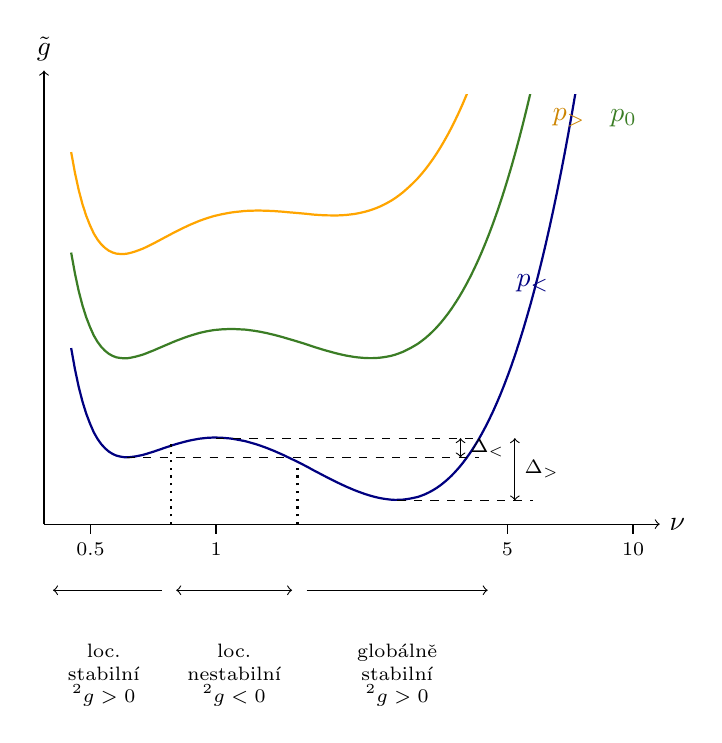
\begin{tikzpicture}[x=2.3cm,y=6cm]
  % osy (x = ln nu)
  \begin{scope}
    \clip (-0.95,-4.46) rectangle (2.4,-3.55);
    \draw[Orange,thick,domain=-0.8:2.3,samples=150]
      plot (\x,{exp(\x)*0.7 - 3/exp(\x) - 2.4*(4*ln(0.9) + ln(3*exp(\x)-1) - ln(0.7))});
    \draw[OliveGreen,thick,domain=-0.8:2.3,samples=150]
      plot (\x,{exp(\x)*0.647 - 3/exp(\x) - 2.4*(4*ln(0.9) + ln(3*exp(\x)-1) - ln(0.647))});
    \draw[NavyBlue,thick,domain=-0.8:2.3,samples=150]
      plot (\x,{exp(\x)*0.6 - 3/exp(\x) - 2.4*(4*ln(0.9) + ln(3*exp(\x)-1) - ln(0.6))});
  \end{scope}
  \draw[->] (-0.95,-4.46) -- (2.45,-4.46) node[right] {$\nu$};
  \draw[->] (-0.95,-4.46) -- (-0.95,-3.5) node[above] {$\tilde g$};
  \foreach \v/\l in {0.5/0.5, 1/1, 5/5, 10/10} \draw ({ln(\v)},-4.46) -- ({ln(\v)},-4.48) node[below] {\scriptsize\l};
  \node[Orange!80!black] at (1.95,-3.6) {$p_>$};
  \node[OliveGreen] at (2.25,-3.6) {$p_0$};
  \node[NavyBlue] at (1.75,-3.95) {$p_<$};
  % bariéry
  \draw[dashed] (0,-4.278) -- (1.45,-4.278);
  \draw[dashed] ({ln(0.61)},-4.319) -- (1.45,-4.319);
  \draw[dashed] ({ln(2.72)},-4.41) -- (1.75,-4.41);
  \draw[<->] (1.35,-4.278) -- (1.35,-4.319) node[midway,right] {\scriptsize$\Delta_<$};
  \draw[<->] (1.65,-4.278) -- (1.65,-4.41) node[midway,right] {\scriptsize$\Delta_>$};
  % oblasti stability (inflexní body)
  \draw[dotted,thick] (-0.25,-4.46) -- (-0.25,-4.29);
  \draw[dotted,thick] (0.45,-4.46) -- (0.45,-4.33);
  \draw[<-] (-0.9,-4.6) -- (-0.3,-4.6);
  \draw[<->] (-0.22,-4.6) -- (0.42,-4.6);
  \draw[->] (0.5,-4.6) -- (1.5,-4.6);
  \node[align=center,font=\scriptsize] at (-0.62,-4.78) {loc.\\ stabilní\\ $\dd^2g > 0$};
  \node[align=center,font=\scriptsize] at (0.1,-4.78) {loc.\\ nestabilní\\ $\dd^2g < 0$};
  \node[align=center,font=\scriptsize] at (1,-4.78) {globálně\\ stabilní\\ $\dd^2g > 0$};
\end{tikzpicture}
\hspace{0.3cm}
\begin{minipage}[b]{0.3\textwidth}
$T = 0{,}9\,T_c$ \\[4pt]
{\color{OliveGreen}$p_0 = 0{,}647\,p_c$} \\[4pt]
$p_> > p_0$ \\[2pt]
$p_< < p_0$ \\[8pt]
{\small $\Delta_<$ \dots\ bariéra z loc.\ minima do glob. \\
$\Delta_>$ \dots\ bariéra glob.\ $\to$ loc.\ min \\[2pt]
$\exp(-\Delta_>) \ll \exp(-\Delta_<)$} \\[6pt]
{\color{NavyBlue}\small $\bullet$ $v_1$ je extenzivní \\ $\Rightarrow$ stabilní $g$ je konvexní!}
\end{minipage}
\end{center}

\begin{itemize}
  \item levé minimum -- kapalná fáze \\
        \hspace*{6em} -- $\nu_{eq}$ málo závislé na tlaku
  \item pravé minimum -- plynná fáze \\
        \hspace*{8em} $\nu_{eq}(p\downarrow)\nearrow$
  \item v oblasti loc.\ stability je rovnovážný systém stabilní vůči infinit.\ fluktuacím $\delta$ \\
        $\Rightarrow$ je možné dosáhnout \kw{podchlazení / přehřátí} \\
        {\color{NavyBlue}\small (tj.\ systém zůstává v loc.\ minimu, které není minimem globálním)}
\end{itemize}

%----------------------------------------------------------------------
\strana{L7-4}
\begin{itemize}
  \item k přechodu mezi fázemi -- překonání bariéry -- je třeba velká fluktuace $\Delta$ \\
  $\to$ pravděpodobnost takové fluktuace je úměrná $e^{-\Delta}$ (viz nerovnovážná stat.\ fyzika) \\
  $\Rightarrow$ jakmile systém přejde do globálního minima, přechod zpět je mnohem méně pravděpodobný
  $\Rightarrow$ systém se nachází téměř veškerý čas v globálně stabilní fázi
\end{itemize}

\subsection{Van der Waalsův plyn a nestabilní izotermy}

\begin{center}
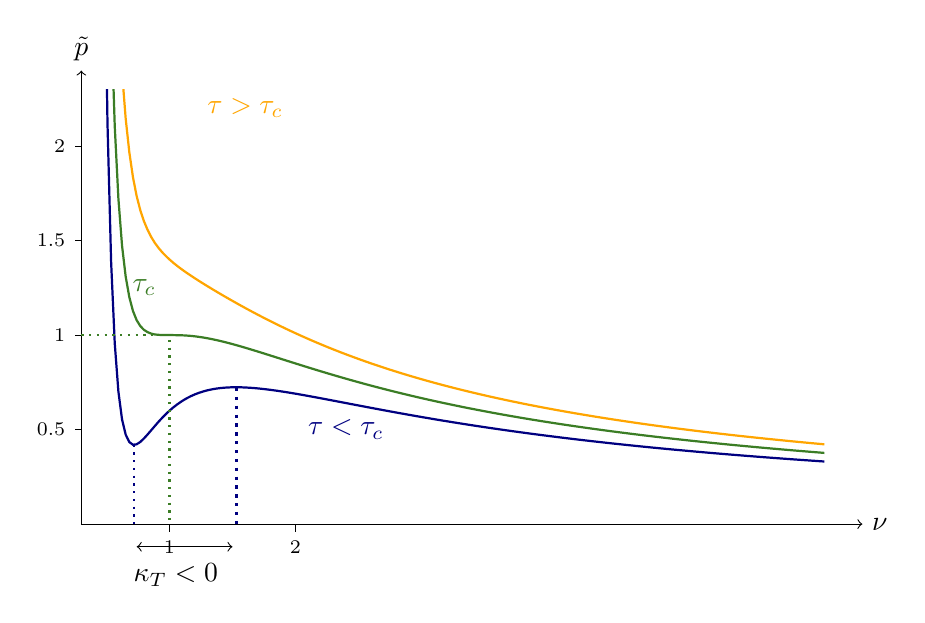
\begin{tikzpicture}[x=1.6cm,y=2.4cm]
  \begin{scope}
    \clip (0.3,0) rectangle (6.3,2.3);
    \draw[Orange,thick,domain=0.45:6.2,samples=200] plot (\x,{8*1.1/(3*\x-1) - 3/(\x*\x)});
    \draw[OliveGreen,thick,domain=0.45:6.2,samples=200] plot (\x,{8*1/(3*\x-1) - 3/(\x*\x)});
    \draw[NavyBlue,thick,domain=0.45:6.2,samples=200] plot (\x,{8*0.9/(3*\x-1) - 3/(\x*\x)});
  \end{scope}
  \draw[->] (0.3,0) -- (6.5,0) node[right] {$\nu$};
  \draw[->] (0.3,0) -- (0.3,2.4) node[above] {$\tilde p$};
  \foreach \y in {0.5,1,1.5,2} \draw (0.3,\y) -- (0.25,\y) node[left] {\scriptsize\y};
  \foreach \x in {1,2} \draw (\x,0) -- (\x,-0.04) node[below] {\scriptsize\x};
  \node[Orange] at (1.6,2.2) {$\tau > \tau_c$};
  \node[OliveGreen] at (0.8,1.25) {$\tau_c$};
  \node[NavyBlue] at (2.4,0.5) {$\tau < \tau_c$};
  \draw[OliveGreen,dotted,thick] (0.3,1) -- (1,1) -- (1,0);
  \draw[NavyBlue,dotted,thick] (0.72,0.42) -- (0.72,0);
  \draw[NavyBlue,dotted,very thick] (1.53,0.72) -- (1.53,0);
  \draw[<->] (0.74,-0.12) -- (1.5,-0.12);
  \node at (1.05,-0.27) {$\kappa_T < 0$};
\end{tikzpicture}
\hspace{0.5cm}
\begin{minipage}[b]{0.3\textwidth}
\[ p = \frac{RT}{v - b} - \frac{a}{v^2} \]
\[ \Updownarrow \]
\[ \vzorec{\tilde p = \frac{8\tau}{3\nu - 1} - \frac{3}{\nu^2}} \]
\vspace{1.5cm}
\end{minipage}
\end{center}

\begin{itemize}
  \item nad $\tau_c$ se s rostoucí teplotou vdW izotermy blíží ideálnímu plynu -- hyperboly $p = \frac{RT}{v}$
  \item pod $\tau_c$ existuje \uv{nestabilní} oblast
        \[ \Big(\pdv{p}{v}\Big) > 0 \quad\Leftrightarrow\quad \text{\pozor{$\kappa_T < 0$\ !}} \]
  \item $\tau = \tau_c$: minimum a maximum splynou v inflexní bod, \ $\kappa_T(T_c,p_c)\to\infty$
\end{itemize}

%----------------------------------------------------------------------
\strana{L7-5}
\begin{itemize}
  \item \underline{volná energie} \quad $f_{vdW}(\tau < \tau_c,\nu)$
\end{itemize}

\begin{center}
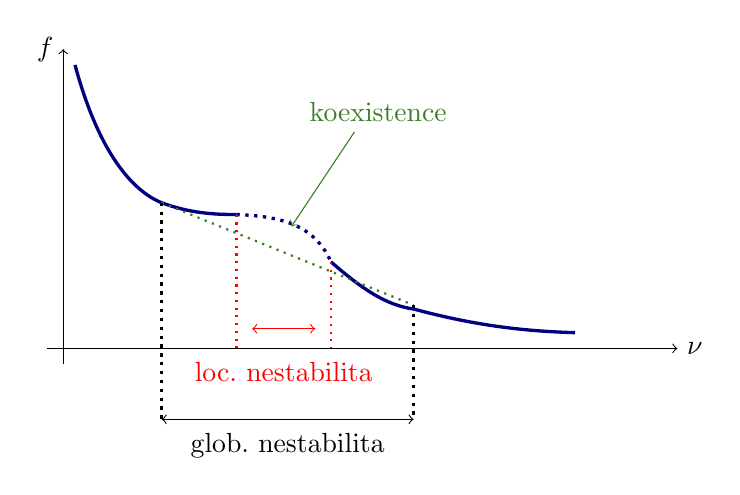
\begin{tikzpicture}[x=1cm,y=1cm]
  \draw[->] (-0.2,0) -- (7.8,0) node[right] {$\nu$};
  \draw[->] (0,-0.2) -- (0,3.8) node[left] {$f$};
  % stabilní části
  \draw[NavyBlue,very thick] (0.15,3.6) .. controls (0.5,2.3) and (1,1.95) .. (1.25,1.85)
        .. controls (1.6,1.72) and (1.9,1.7) .. (2.2,1.7);
  \draw[NavyBlue,very thick,dotted] (2.2,1.7) .. controls (2.8,1.68) and (3.2,1.55) .. (3.4,1.1);
  \draw[NavyBlue,very thick] (3.4,1.1) .. controls (3.8,0.75) and (4.1,0.55) .. (4.45,0.5)
        .. controls (5.2,0.3) and (5.8,0.22) .. (6.5,0.2);
  % společná tečna
  \draw[OliveGreen,thick,dotted] (1.25,1.85) -- (4.45,0.55);
  \node[OliveGreen] at (4,3) {koexistence};
  \draw[OliveGreen,->] (3.7,2.75) -- (2.9,1.55);
  % lokální nestabilita
  \draw[Red,dotted,thick] (2.2,1.7) -- (2.2,0);
  \draw[Red,dotted,thick] (3.4,1.1) -- (3.4,0);
  \draw[Red,<->] (2.4,0.25) -- (3.2,0.25);
  \node[Red,below] at (2.8,-0.05) {loc.\ nestabilita};
  % globální nestabilita
  \draw[dotted,very thick] (1.25,1.85) -- (1.25,-0.9);
  \draw[dotted,very thick] (4.45,0.55) -- (4.45,-0.9);
  \draw[<->] (1.25,-0.9) -- (4.45,-0.9);
  \node[below] at (2.85,-0.95) {glob.\ nestabilita};
\end{tikzpicture}
\hspace{0.3cm}
\begin{minipage}[b]{0.32\textwidth}
$\to$ vyhazuje oblast globální a loc.\ nestability \\[6pt]
{\color{OliveGreen}$\to$ stabilní $f(\tau,\nu)$ získáme definicí $f$ jako obálky tečných nadploch}
\vspace{1cm}
\end{minipage}
\end{center}

\begin{itemize}
  \item fázový přechod souvisí s nestabilní částí izotermy$/f(\tau,\nu)$ a existencí více řešení rovnice $\nu = \nu(\tau,\tilde p)$
\end{itemize}

\begin{center}
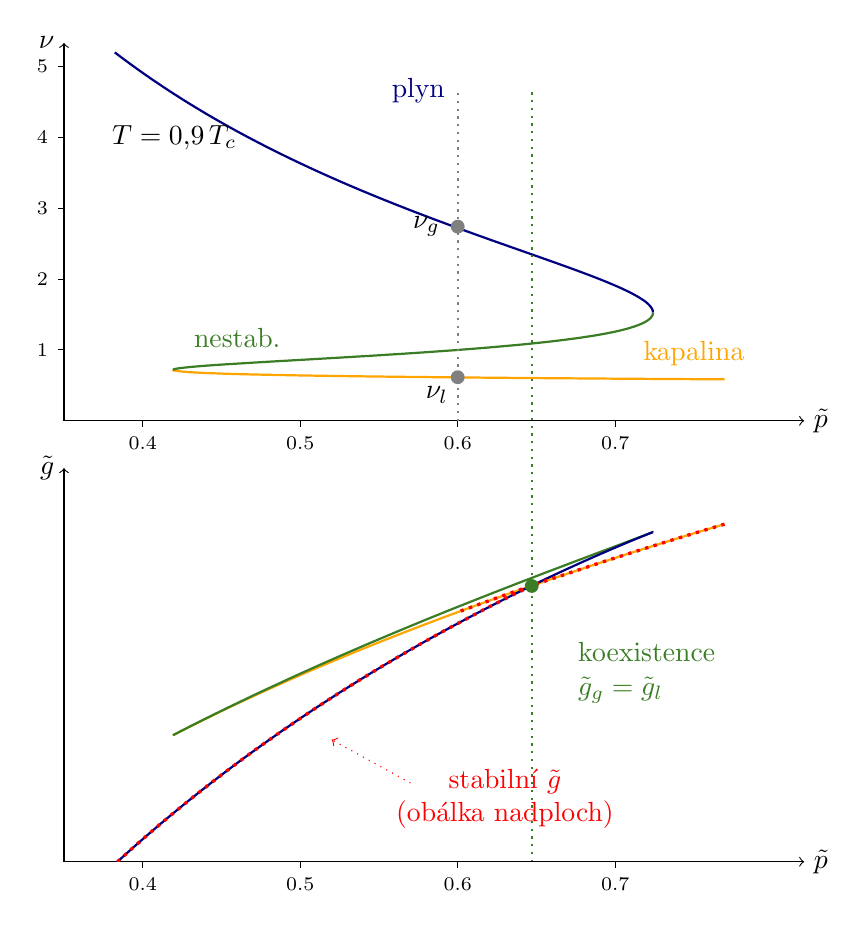
\begin{tikzpicture}[x=1cm,y=1cm,
    declare function={P(\t)=8*0.9/(3*\t-1)-3/(\t*\t);
                      G(\t)=\t*P(\t)-3/\t-2.4*(4*ln(0.9)+ln(3*\t-1)-ln(P(\t)));}]
  %--- horní graf: nu(p) ---
  \begin{scope}[yshift=5.6cm]
    \draw[->] (0,0) -- (9.4,0) node[right] {$\tilde p$};
    \draw[->] (0,0) -- (0,4.8) node[left] {$\nu$};
    \foreach \p in {0.4,0.5,0.6,0.7} \draw ({(\p-0.35)*20},0) -- ({(\p-0.35)*20},-0.08) node[below] {\scriptsize\p};
    \foreach \v in {1,2,3,4,5} \draw (0,{\v*0.9}) -- (-0.08,{\v*0.9}) node[left] {\scriptsize\v};
    \draw[Orange,thick,variable=\t,domain=0.585:0.719,samples=60] plot ({(P(\t)-0.35)*20},{\t*0.9});
    \draw[OliveGreen,thick,variable=\t,domain=0.719:1.529,samples=80] plot ({(P(\t)-0.35)*20},{\t*0.9});
    \draw[NavyBlue,thick,variable=\t,domain=1.529:5.2,samples=120] plot ({(P(\t)-0.35)*20},{\t*0.9});
    \node at (1.4,3.6) {$T = 0{,}9\,T_c$};
    \node[NavyBlue] at (4.5,4.2) {plyn};
    \node[OliveGreen] at (2.2,1.05) {nestab.};
    \node[Orange] at (8,0.85) {kapalina};
    % p = 0.6
    \draw[gray,dotted,thick] (5,0) -- (5,4.2);
    \fill[gray] (5,{2.74*0.9}) circle (2.5pt) node[black,left=3pt] {$\nu_g$};
    \fill[gray] (5,{0.615*0.9}) circle (2.5pt) node[black,below left] {$\nu_l$};
    % koexistence
    \draw[OliveGreen,dotted,thick] ({(0.647-0.35)*20},-5.6) -- ({(0.647-0.35)*20},4.2);
  \end{scope}
  %--- dolní graf: g(p) ---
  \begin{scope}
    \draw[->] (0,0) -- (9.4,0) node[right] {$\tilde p$};
    \draw[->] (0,0) -- (0,5) node[left] {$\tilde g$};
    \foreach \p in {0.4,0.5,0.6,0.7} \draw ({(\p-0.35)*20},0) -- ({(\p-0.35)*20},-0.08) node[below] {\scriptsize\p};
    \begin{scope}
      \clip (0,0) rectangle (9.4,5);
      \draw[Orange,thick,variable=\t,domain=0.585:0.719,samples=60] plot ({(P(\t)-0.35)*20},{(G(\t)+6.3)*1.6});
      \draw[OliveGreen,thick,variable=\t,domain=0.719:1.529,samples=80] plot ({(P(\t)-0.35)*20},{(G(\t)+6.3)*1.6});
      \draw[NavyBlue,thick,variable=\t,domain=1.529:5.2,samples=120] plot ({(P(\t)-0.35)*20},{(G(\t)+6.3)*1.6});
      % stabilní g (obálka)
      \draw[Red,dotted,very thick,variable=\t,domain=2.35:5.2,samples=80] plot ({(P(\t)-0.35)*20},{(G(\t)+6.3)*1.6});
      \draw[Red,dotted,very thick,variable=\t,domain=0.585:0.612,samples=30] plot ({(P(\t)-0.35)*20},{(G(\t)+6.3)*1.6});
    \end{scope}
    \fill[OliveGreen] ({(0.647-0.35)*20},{(-4.111+6.3)*1.6}) circle (2.5pt);
    \node[OliveGreen,align=left] at (7.4,2.4) {koexistence\\ $\tilde g_g = \tilde g_l$};
    \node[Red,align=center] at (5.6,0.8) {stabilní $\tilde g$\\ (obálka nadploch)};
    \draw[Red,dotted,->] (4.4,1.0) -- (3.4,1.55);
  \end{scope}
\end{tikzpicture}
\hspace{0.2cm}
\begin{minipage}[b]{0.3\textwidth}
\fbox{\parbox{0.95\linewidth}{
1) $\exists$ řešení $\nu = \nu(\tau,\tilde p)$ (pouze tam, kde jsou $\mathbb{R}$)

\medskip
2) odpovídající $\exists$ větve
{\small $\tilde g(\tau,\tilde p) = f\big(\tau,\nu(\tau,\tilde p)\big)$ \\ \hspace*{3em} $+\ \nu(\tau,\tilde p)\,\tilde p$}

\medskip

3) vidíme {\color{NavyBlue}plyn}, {\color{Orange}kapalinu} i {\color{OliveGreen}nestabilní větev}

\medskip
$\bullet$ \kw{stabilní fáze odpovídá nižšímu $\tilde g(\tau,\tilde p)$}
}}
\vspace{1.5cm}
\end{minipage}
\end{center}

%----------------------------------------------------------------------
\strana{L7-6}
\subsection{Koexistence fází -- Maxwellova konstrukce}
\begin{itemize}[nosep]
  \item $g(T,p) = \dfrac{G(T,p,N)}{N} = /\text{Euler}/ = \mu(T,p)$
  \item $\dd g = -s\,\dd T + v\,\dd p = /T = \text{konst}/ = v(p)\,\dd p$
\end{itemize}

\begin{center}
\begin{tikzpicture}[x=1cm,y=1cm,
    declare function={P(\t)=8*0.9/(3*\t-1)-3/(\t*\t);
                      G(\t)=\t*P(\t)-3/\t-2.4*(4*ln(0.9)+ln(3*\t-1)-ln(P(\t)));}]
  %--- horní graf: v(p) ---
  \begin{scope}[yshift=5.6cm]
    \draw[->] (0,0) -- (9.4,0) node[right] {$p$};
    \draw[->] (0,0) -- (0,4.9) node[left] {$v$};
    \foreach \p in {0.4,0.5,0.6,0.7} \draw ({(\p-0.35)*20},0) -- ({(\p-0.35)*20},-0.08) node[below] {\scriptsize\p};
    % šrafované plochy
    \fill[pattern=north east lines] plot[variable=\t,domain=2.349:1.529,samples=40] ({(P(\t)-0.35)*20},{\t*0.9})
        -- plot[variable=\t,domain=1.529:1.0905,samples=40] ({(P(\t)-0.35)*20},{\t*0.9}) -- cycle;
    \fill[pattern=north west lines] plot[variable=\t,domain=1.0905:0.719,samples=40] ({(P(\t)-0.35)*20},{\t*0.9})
        -- plot[variable=\t,domain=0.719:0.6034,samples=40] ({(P(\t)-0.35)*20},{\t*0.9}) -- cycle;
    \draw[Orange,thick,variable=\t,domain=0.584:0.719,samples=60] plot ({(P(\t)-0.35)*20},{\t*0.9});
    \draw[OliveGreen,thick,variable=\t,domain=0.719:1.529,samples=80] plot ({(P(\t)-0.35)*20},{\t*0.9});
    \draw[NavyBlue,thick,variable=\t,domain=1.529:5,samples=120] plot ({(P(\t)-0.35)*20},{\t*0.9});
    \draw[dotted,very thick] ({(0.647-0.35)*20},0) -- ({(0.647-0.35)*20},4.2);
    % body
    \node[above left] at ({(0.394-0.35)*20},4.5) {\small A};
    \node[above right] at ({(0.42-0.35)*20},{4.61*0.9}) {\small B};
    \node[above right] at ({(0.647-0.35)*20},{2.349*0.9}) {\small C};
    \node[right] at ({(0.724-0.35)*20},{1.529*0.9}) {\small D};
    \node[left] at ({(0.647-0.35)*20},{1.0905*0.9}) {\small E};
    \node[left] at ({(0.42-0.35)*20},{0.719*0.9}) {\small F};
    \node[below right] at ({(0.647-0.35)*20},{0.6034*0.9}) {\small G};
    \node[below] at ({(0.724-0.35)*20},{0.5912*0.9}) {\small H};
    \node[below] at ({(0.78-0.35)*20},{0.5838*0.9}) {\small I};
    \node at (6.9,1.75) {I};
    \node at (5.0,0.78) {II};
    \node at (7.5,2.9) {$A_I$}; \draw[->] (7.3,2.75) -- (6.8,1.95);
    \node at (3.2,1.6) {$A_{II}$}; \draw[->] (3.4,1.4) -- (3.8,0.8);
  \end{scope}
  %--- dolní graf: g(p) ---
  \begin{scope}
    \draw[->] (0,0) -- (9.4,0) node[right] {$p$};
    \draw[->] (0,0) -- (0,5) node[left] {$g$};
    \foreach \p in {0.4,0.5,0.6,0.7} \draw ({(\p-0.35)*20},0) -- ({(\p-0.35)*20},-0.08) node[below] {\scriptsize\p};
    \begin{scope}
      \clip (0,0) rectangle (9.4,5);
      \draw[Orange,thick,variable=\t,domain=0.584:0.719,samples=60] plot ({(P(\t)-0.35)*20},{(G(\t)+6.3)*1.6});
      \draw[OliveGreen,thick,variable=\t,domain=0.719:1.529,samples=80] plot ({(P(\t)-0.35)*20},{(G(\t)+6.3)*1.6});
      \draw[NavyBlue,thick,variable=\t,domain=1.529:5,samples=120] plot ({(P(\t)-0.35)*20},{(G(\t)+6.3)*1.6});
    \end{scope}
    \draw[dotted,very thick] ({(0.647-0.35)*20},{(-4.111+6.3)*1.6}) -- ({(0.647-0.35)*20},5);
    \node[below right] at ({(0.647-0.35)*20},{(-4.111+6.3)*1.6}) {\small C;G};
    \node[above] at ({(0.724-0.35)*20},{(G(1.529)+6.3)*1.6}) {\small D};
    \node[above left] at ({(0.647-0.35)*20},{(G(1.0905)+6.3)*1.6}) {\small E};
    \node[above left] at ({(0.42-0.35)*20},{(G(0.719)+6.3)*1.6}) {\small F};
    \node[below] at ({(0.724-0.35)*20},{(G(0.5912)+6.3)*1.6}) {\small H};
    \node[below] at ({(0.78-0.35)*20},{(G(0.5838)+6.3)*1.6}) {\small I};
    \node[below right] at ({(0.42-0.35)*20},{(G(4.61)+6.3)*1.6}) {\small B};
    \node[below left] at ({(0.394-0.35)*20},{(G(5)+6.3)*1.6}) {\small A};
  \end{scope}
\end{tikzpicture}
\hspace{0.1cm}
\begin{minipage}[b]{0.3\textwidth}
\[ g(p) - g(A) = \int_A^p v(p)\,\dd p \]
\vspace{0.5cm}

$\bullet$ \underline{koexistence:}
\[ g(C) = g(G) \]
\[ \Updownarrow \]
\[ \int_C^G v\,\dd p = 0 \]
\[ \Updownarrow \]
\vspace{4.5cm}
\end{minipage}
\end{center}

\[
  \underbrace{\int_C^D v\,\dd p}_{\dd p > 0} + \underbrace{\int_D^E v\,\dd p}_{\dd p < 0}
  + \underbrace{\int_E^F v\,\dd p}_{\dd p < 0} + \underbrace{\int_F^G v\,\dd p}_{\dd p > 0} = 0
\]
\vspace{-6pt}
\[
  \hspace{-2.2cm}\underbrace{\hspace{3.6cm}}_{A_I}\qquad\underbrace{\hspace{3.6cm}}_{-A_{II}}
\]

$\to$ podmínka na koexistenci je rovnost ploch
\[
  \vzorec{A_I = A_{II}} \quad\Rightarrow\quad p_{ce} = p_{ce}(T)
\]

\begin{center}
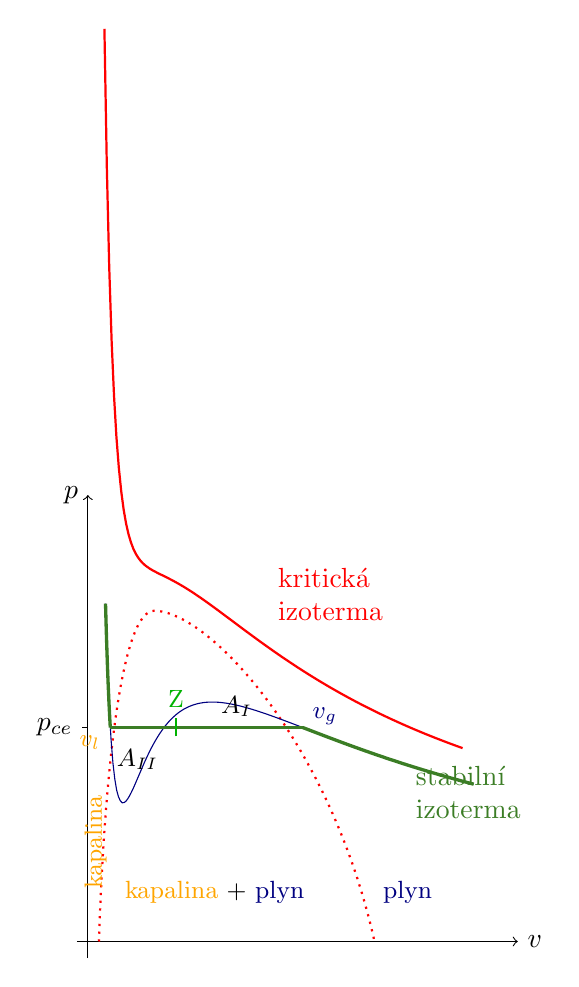
\begin{tikzpicture}[x=1.4cm,y=4.2cm]
  % p-v diagram
  \draw[->] (0.3,0) -- (4.3,0) node[right] {$v$};
  \draw[->] (0.4,-0.05) -- (0.4,1.35) node[left] {$p$};
  % kritická izoterma
  \draw[Red,thick,domain=0.55:3.8,samples=150] plot (\x,{8*1.03/(3*\x-1)-3/(\x*\x)});
  \node[Red,align=left] at (2.6,1.05) {kritická\\ izoterma};
  % binodála
  \draw[Red,dotted,thick] (0.5,0) .. controls (0.55,0.5) and (0.7,1.0) .. (1,1.0)
      .. controls (1.5,1.0) and (2.6,0.6) .. (3.0,0);
  % vdW izoterma
  \draw[NavyBlue,domain=0.56:3.9,samples=200] plot (\x,{8*0.9/(3*\x-1)-3/(\x*\x)});
  % stabilní izoterma
  \draw[OliveGreen,very thick,domain=0.56:0.6034,samples=20] plot (\x,{8*0.9/(3*\x-1)-3/(\x*\x)});
  \draw[OliveGreen,very thick] (0.6034,0.647) -- (2.349,0.647);
  \draw[OliveGreen,very thick,domain=2.349:3.9,samples=60] plot (\x,{8*0.9/(3*\x-1)-3/(\x*\x)});
  \draw[green!70!black,thick] (1.2,0.62) -- (1.2,0.675) node[above] {\small Z};
  \draw (0.4,0.647) -- (0.35,0.647) node[left] {$p_{ce}$};
  \node at (0.85,0.55) {\small $A_{II}$};
  \node at (1.75,0.71) {\small $A_I$};
  \node[Orange,left] at (0.6,0.6) {\small $v_l$};
  \node[NavyBlue,right] at (2.35,0.68) {\small $v_g$};
  \node[Orange,rotate=90] at (0.47,0.3) {\small kapalina};
  \node at (1.55,0.15) {\small{\color{Orange}kapalina} + {\color{NavyBlue}plyn}};
  \node[NavyBlue] at (3.3,0.15) {\small plyn};
  \node[OliveGreen,align=left] at (3.85,0.45) {stabilní\\ izoterma};
\end{tikzpicture}
\quad {\color{OliveGreen}$\longleftrightarrow$} \quad
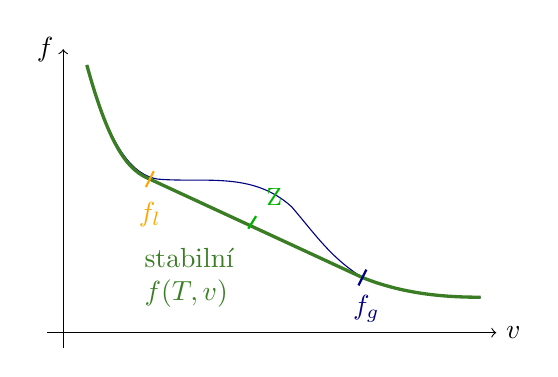
\begin{tikzpicture}[x=1cm,y=1cm]
  \draw[->] (-0.2,0) -- (5.5,0) node[right] {$v$};
  \draw[->] (0,-0.2) -- (0,3.6) node[left] {$f$};
  \draw[NavyBlue] (0.3,3.4) .. controls (0.6,2.3) and (0.9,2.0) .. (1.2,1.95)
      .. controls (1.8,1.9) and (2.4,2.05) .. (2.9,1.6) .. controls (3.2,1.25) and (3.4,0.95) .. (3.8,0.7)
      .. controls (4.3,0.5) and (4.8,0.45) .. (5.3,0.45);
  \draw[OliveGreen,very thick] (0.3,3.4) .. controls (0.6,2.3) and (0.85,2.05) .. (1.1,1.95)
      -- (3.8,0.7) .. controls (4.3,0.5) and (4.8,0.45) .. (5.3,0.45);
  \draw[Orange,thick] (1.05,1.85) -- (1.15,2.05);
  \node[Orange] at (1.1,1.5) {$f_l$};
  \draw[green!70!black,thick] (2.35,1.32) -- (2.45,1.48) node[above right] {\small Z};
  \draw[NavyBlue,thick] (3.75,0.6) -- (3.85,0.8);
  \node[NavyBlue] at (3.85,0.3) {$f_g$};
  \node[OliveGreen,align=left] at (1.6,0.7) {stabilní\\ $f(T,v)$};
\end{tikzpicture}
\end{center}

%----------------------------------------------------------------------
\strana{L7-7}
\begin{itemize}
  \item zjišťujeme, že pro danou teplotu mohou obě fáze koexistovat pouze při konkrétním tlaku $p_{ce}(T)$, který je dán rovnicí
  \[ g_g(T,p_{ce}) = g_l(T,p_{ce}) \quad\Leftrightarrow\quad \vzorec{\mu_g(T,p_{ce}) = \mu_l(T,p_{ce})} \]
  \item mol.\ frakce fází jsou dány \uv{\kw{pákovým pravidlem}} (lever rule)
  \begin{itemize}[nosep]
    \item[$\to$] nechť celkový počet částic je $N$ a celkový objem je $V$
    \item[$\to$] $x_i = \dfrac{N_i}{N}$ jsou mol.\ frakce (koncentrace) fází
    \item[$\to$] $N_g + N_l = N \ \Leftrightarrow\ x_g + x_l = 1$
    \item[$\Rightarrow$] $V = Nv = N_gv_g + N_lv_l = N(x_gv_g + x_lv_l)$
  \end{itemize}
  \[
    \Rightarrow /x_g = 1 - x_l/ \ \Rightarrow\ \vzorec{x_l = \frac{v_g - v}{v_g - v_l}}
  \]
  \hfill
  \begin{minipage}{0.45\textwidth}
  $\bullet$ LEVER RULE \\
  $\bullet$ objem $v$ odpovídá obecnému bodu {\color{green!70!black}Z} v obrázku výše
  \end{minipage}
  \item z konstrukce vyplývá, že izotermickým snižováním objemu neměníme tlak, ale zvyšujeme podíl kapalné složky
  \item analog.\ pákové pravidlo dostáváme pro libovolnou ext.\ veličinu $X$, která se při fázovém přechodu skokově mění
  \[ x_l = \frac{X_g - X}{X_g - X_l} \]
  \item podmínka $\mu_1(T,p) = \mu_2(T,p)$ je \underline{podmínka rovnováhy při výměně hmoty} mezi fázemi:
  \begin{itemize}[nosep]
    \item $T,p$ konst $\Leftrightarrow$ $[\Delta G]_{T,p} > 0$
    \item Euler: $G = \sum_i\mu_iN_i$ \ \& \ $\dd N_2 = -\dd N_1$ \ $\Rightarrow$ \ $\dd G = (\mu_1 - \mu_2)\,\dd N_1 = 0$
  \end{itemize}
\end{itemize}
{\color{NavyBlue}
$\bullet$ Co tu dělám: $G = G(T,p,N_1,N_2)$ \quad $N_i$ -- počet částic v $i$-té fázi \\
\hspace*{1em} $\hookrightarrow$ dává to smysl? \quad $\bullet$ pro obecné $T,p$ je $N_i = N\delta_{ik}$ \\
\hspace*{1em} $\to$ $G = \mu_1(T,p,N_1)N_1 + \mu_2(T,p,N_2)N_2$ jsou ony 2 větve $G$, typ.\ se realizuje jen jedna \\
\hspace*{1em} $\to$ $\mu_1 \neq \mu_1(N_2)$, neboť vlastnosti fáze nezávisí na přítomnosti druhé fáze (není to směs, předp.\ zanedbatelnou interakci na rozhraní)}

%----------------------------------------------------------------------
\strana{L7-8}
{\color{NavyBlue}$\bullet$ je to lépe vidět na složeném systému?}

\begin{center}
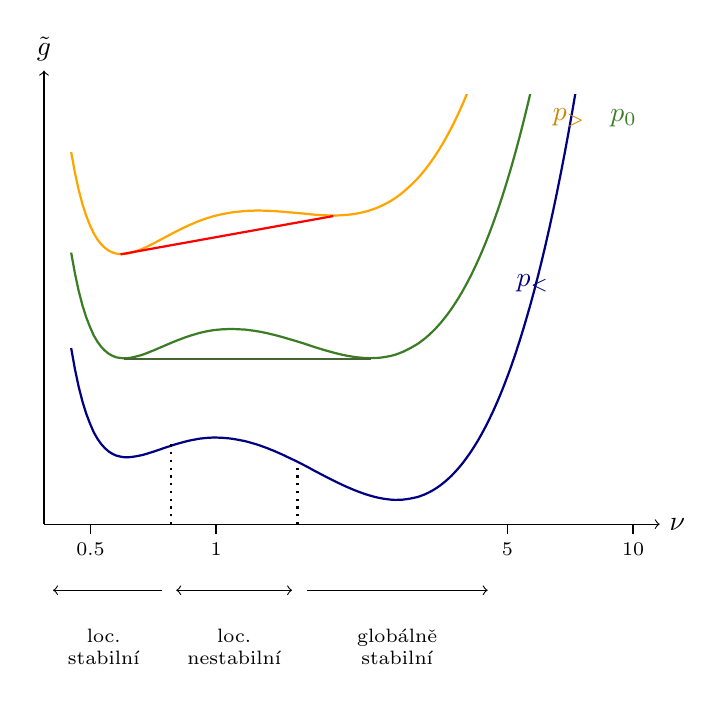
\begin{tikzpicture}[x=2.3cm,y=6cm]
  \begin{scope}
    \clip (-0.95,-4.46) rectangle (2.4,-3.55);
    \draw[Orange,thick,domain=-0.8:2.3,samples=150]
      plot (\x,{exp(\x)*0.7 - 3/exp(\x) - 2.4*(4*ln(0.9) + ln(3*exp(\x)-1) - ln(0.7))});
    \draw[OliveGreen,thick,domain=-0.8:2.3,samples=150]
      plot (\x,{exp(\x)*0.647 - 3/exp(\x) - 2.4*(4*ln(0.9) + ln(3*exp(\x)-1) - ln(0.647))});
    \draw[NavyBlue,thick,domain=-0.8:2.3,samples=150]
      plot (\x,{exp(\x)*0.6 - 3/exp(\x) - 2.4*(4*ln(0.9) + ln(3*exp(\x)-1) - ln(0.6))});
  \end{scope}
  % tětivy
  \draw[Red,thick] ({ln(0.59)},-3.889) -- ({ln(1.91)},-3.808);
  \draw[OliveGreen!70!black,thick] ({ln(0.6)},-4.11) -- ({ln(2.35)},-4.11);
  \draw[->] (-0.95,-4.46) -- (2.45,-4.46) node[right] {$\nu$};
  \draw[->] (-0.95,-4.46) -- (-0.95,-3.5) node[above] {$\tilde g$};
  \foreach \v/\l in {0.5/0.5, 1/1, 5/5, 10/10} \draw ({ln(\v)},-4.46) -- ({ln(\v)},-4.48) node[below] {\scriptsize\l};
  \node[Orange!80!black] at (1.95,-3.6) {$p_>$};
  \node[OliveGreen] at (2.25,-3.6) {$p_0$};
  \node[NavyBlue] at (1.75,-3.95) {$p_<$};
  \draw[dotted,thick] (-0.25,-4.46) -- (-0.25,-4.29);
  \draw[dotted,thick] (0.45,-4.46) -- (0.45,-4.33);
  \draw[<-] (-0.9,-4.6) -- (-0.3,-4.6);
  \draw[<->] (-0.22,-4.6) -- (0.42,-4.6);
  \draw[->] (0.5,-4.6) -- (1.5,-4.6);
  \node[align=center,font=\scriptsize] at (-0.62,-4.72) {loc.\\ stabilní};
  \node[align=center,font=\scriptsize] at (0.1,-4.72) {loc.\\ nestabilní};
  \node[align=center,font=\scriptsize] at (1,-4.72) {globálně\\ stabilní};
\end{tikzpicture}
\end{center}

{\color{NavyBlue}
$\bullet$ zde \textcolor{Red}{červeně} \ $G = G(\tau,\tilde p,N_{id},N_{w};\nu) = G(\tau,\tilde p,N_{id},N_{w};x_l)$

$\bullet$ co nyní udělám je, že přejdu ke
\begin{align*}
  G = G(\tau,\tilde p,N_{id},N_w) &= G(\tau,\tilde p,N_{id},N_w;\nu_{eq}) \\
  &= x_l\,G_l(\tau,\tilde p,N_{id},N_w) + (1 - x_l)\,G_g(\tau,\tilde p,N_{id},N_w)
\end{align*}
\quad $x_l = \dfrac{N_l}{N_w}$ \quad \dots\ $x_l$ je $1$ pro $p_>$ a $0$ pro $p_<$, \\
\hspace*{9.4em} ale $x_l\in(0,1)$ pro $p = p_0$

$\bullet$ abych ale viděl význam $G_{l/g}$ jakožto chem.\ potenciálu, musel bych si tam přidat $f_{vdW}\to N_w f_{vdW}$ \\
\hspace*{1em} a ideálně taky $f_{id}\to N_{id} f_{id}$}

%----------------------------------------------------------------------
\strana{L7-9}
\subsection{Fázové přechody I.\ druhu obecně}
\begin{itemize}
  \item fázové přechody nastávají v bodech stav.\ prostoru, ve kterých stavové funkce nejsou analytické
        {\color{NavyBlue}\itshape\small * druhé derivace TD potenciálu nulové nebo nekonečné (nehladkost $G$)}
  \item typicky změna skupenství nebo strukturní změny krystal.\ mřížek
  \item přechody I.\ druhu jsou charakterizovány rozdíly {\small\itshape hustot} extenzivních veličin v různých fázích tam, kde mohou fáze koexistovat (křivky/nadplochy) koexistence:
\end{itemize}

\begin{minipage}{0.38\textwidth}
\[ \mu_1(T,p) = \mu_2(T,p): \]
{\color{NavyBlue}\itshape\small existuje interval extenzivní proměnné (zde $V$, mezi $V_g$ a $V_l$), ve kterém mohou fáze koexistovat}
\end{minipage}
\begin{minipage}{0.6\textwidth}
1) $s_1(T,p)\neq s_2(T,p)$, \ $v_1(T,p)\neq v_2(T,p)$, \dots \\
\hspace*{1em} $\Rightarrow$ molární hustoty ext.\ veličin se liší (s výjimkou $g$)

\medskip
2) fáze v rovnováze $\Rightarrow$ intenzivní veličiny pro obě fáze stejné
\end{minipage}

\subsubsection*{Křivka koexistence (CC)}
\begin{itemize}
  \item popisuje rovnováhu dvou fází:
  \[ \mu_1(T,p) = \mu_2(T,p) \quad\Rightarrow\quad p = p(T) \]
  \item jeden nezávislý parametr $\Rightarrow$ opravdu se jedná o křivku
  \item $\dd\mu = -s\,\dd T + v\,\dd p$ \ \& \ podél CC musí platit
  \[ \dd\mu_1 = \dd\mu_2 \quad\Rightarrow\quad -s_1\,\dd T + v_1\,\dd p = -s_2\,\dd T + v_2\,\dd p \]
\end{itemize}
\begin{veta}[Sklon křivky koexistence]
\[ \vzorec{\Big(\frac{\dd p}{\dd T}\Big)_{CC} = \frac{s_1 - s_2}{v_1 - v_2} = \frac{\Delta s}{\Delta v}} \]
\end{veta}

\subsubsection*{Latentní teplo (varu, tání, \dots)}
\begin{itemize}
  \item pokud systém obsahuje dvě fáze v rovnováze, dodáváním tepla nezvýšíme teplotu, ale zvýšíme podíl fáze s vyšší molární entropií -- pohybujeme se po vodorovné části stabilní izotermy $p = p(v)$ resp.\ po přímém úseku TD potenciálu
  \item (molární) \kw{latentní teplo}: teplo absorbované nebo uvolněné během fáz.\ přechodu (jednoho molu) látky
\end{itemize}

%----------------------------------------------------------------------
\strana{L7-10}
\begin{itemize}
  \item fáz.\ přechod tedy probíhá za konst.\ $T,p$
  \[ l = T\Delta s = /\dd h = T\,\dd s + v\,\dd p/ = \Delta h \]
  $\to$ var: \ $l = h_g - h_l = T_v(s_g - s_l)$
\end{itemize}
\underline{Pozn:} $T,p = \text{konst}$, $Q > 0$ $\Rightarrow$ efektivně $C_p = +\infty$, neplatí ale ani pro jednu fázi samostatně

$\Rightarrow$ pro CC můžeme psát \underline{Clapeyronovu rovnici}
\begin{veta}[Clapeyronova rovnice]
\[ \vzorec{\Big(\frac{\dd p}{\dd T}\Big)_{CC} = \frac{l}{T\Delta v} = \frac{\Delta h}{T\Delta v}} \]
\end{veta}

\begin{priklad}[Př: vypařování: 1 -- kapalina, 2 -- plyn]
$\to$ pro teploty \underline{dostatečně nízko$^{(*)}$ pod $T_c$} je $v_g \gg v_l$ a plynná fáze je dobře popsána rovnicemi id.\ plynu
\[ \Rightarrow\quad \Delta v = v_g - v_l \simeq v_g \simeq \frac{RT}{p} \]
$\Rightarrow$ \underline{Clausiova--Clapeyronova rovnice}
\[ \vzorec{\frac{\dd p}{\dd T} = \frac{lp}{RT^2}} \]
\begin{minipage}{0.45\textwidth}
$\to$ pro $l \neq l(T)$ lze integrovat
\[ \log\frac{p}{p_0} = -\frac{l}{R}\Big(\frac1T - \frac1{T_0}\Big) \]
\end{minipage}
\begin{minipage}{0.5\textwidth}
$\bullet$ dostáváme vztah mezi latentním teplem a teplotou a tlakem nasycené páry bez odkazu na molární objemy
\end{minipage}
\end{priklad}

\underline{Pozn$^{(*)}$:}
\begin{itemize}[nosep]
  \item[--] trochu kontra-intuitivně zde požadujeme dostatečně nízké teploty, aby byla plynná fáze \uv{ideální}
  \item[--] důvod spočívá v tom, že pro $T\to T_c$ se $v_g$ a $v_l$ přibližují a do plynné fáze systém přechází už v té části izotermy, kde se ještě hodně liší od \uv{ideální} hyperboly
  \item[--] pro $T \gg T_c$ se plyn samozřejmě také chová jako ideální, ale nevykazuje fázový přechod
\end{itemize}

%----------------------------------------------------------------------
\strana{L7-11}
\begin{itemize}
  \item jak dobrá je aproximace $l = \text{konst}$?
  \[ \frac{\dd l}{\dd T} = \frac{\dd}{\dd T}(T\Delta s) = T\frac{\dd(\Delta s)}{\dd T} + \Delta s = T\frac{\dd\Delta s}{\dd T} + \frac{l}{T} \qquad (*) \]
  \begin{itemize}
    \item jsme na CC $\Rightarrow$ $s = s\big(T,p(T)\big)$ \hfill \pozn{$\big(\pdv{v}{T}\big)_p = v\alpha$}
    \[ \frac{\dd\Delta s}{\dd T} = \Big(\pdv{\Delta s}{T}\Big)_p + \Big(\pdv{\Delta s}{p}\Big)_T\frac{\dd p}{\dd T}\Big)_{CC}
       \overset{\text{M.R.}}{=} \frac1T\Delta C_p - \Big(\pdv{\Delta v}{T}\Big)_p\frac{l}{T\Delta v} \]
    \[ \boxed{\frac{\dd\Delta s}{\dd T} = \frac{\Delta C_p}{T} - \frac{\Delta(\alpha v)\,l}{T\Delta v}} \]
    \item spec.\ vypařování: $v_g \gg v_l$ \ \& \ $\alpha_g \gg \alpha_l$, \ $\alpha_g \simeq \frac1T$ (id.\ plyn)
    \[ \Rightarrow\quad \frac{\alpha_gv_g - \alpha_lv_l}{v_g - v_l} = \alpha_g\,\frac{1 - \frac{\alpha_lv_l}{\alpha_gv_g}}{1 - \frac{v_l}{v_g}} \simeq \alpha_g \simeq \frac1T \]
    \[ \Rightarrow\quad \frac{\dd\Delta s}{\dd T} = \frac{\Delta C_p}{T} - \frac{l}{T^2}
       \ \overset{(*)}{\Rightarrow}\ \vzorec{\frac{\dd l}{\dd T}\Big)_{CC} = \Delta C_p} \quad \text{\kw{Kirchhoffova rovnice}} \]
  \end{itemize}
\end{itemize}

\subsection{Fázový diagram}
\begin{itemize}
  \item křivky koexistence různých fází v $T$--$p$ diagramu
  \item $\dfrac{\dd p}{\dd T}\Big)_{CC} = \dfrac{\Delta h}{T\Delta v} = \dfrac{\Delta s}{\Delta v} > 0$, pokud fázi s větší entropií odpovídá větší objem (výjimkou je např.\ led -- voda)
  \item CC kapalina--plyn končí pro vysoké teploty \kw{kritickým bodem} (CP)
  \item u nižších teplot končí \kw{trojným bodem} (TP)
  \[ \mu_g(T,p) = \mu_l(T,p) = \mu_s(T,p) \]
  $\Leftrightarrow$ dvě rovnice pro $T,p$ $\Rightarrow$ řešením je opravdu bod
\end{itemize}

\begin{center}
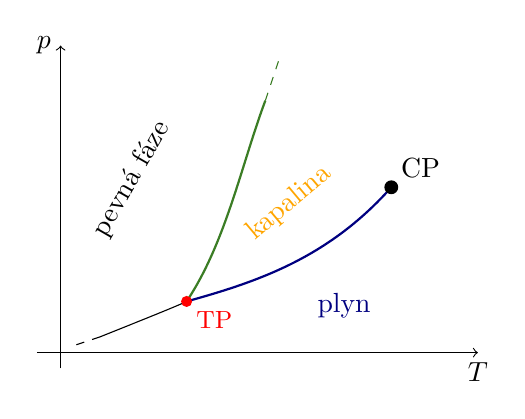
\begin{tikzpicture}[x=1cm,y=1cm]
  \draw[->] (-0.3,0) -- (5.3,0) node[below] {$T$};
  \draw[->] (0,-0.2) -- (0,3.9) node[left] {$p$};
  \draw[dashed] (0.2,0.1) -- (0.5,0.2);
  \draw (0.5,0.2) .. controls (1,0.4) and (1.5,0.6) .. (1.6,0.65);
  \draw[OliveGreen,thick] (1.6,0.65) .. controls (2.1,1.4) and (2.3,2.4) .. (2.6,3.2);
  \draw[OliveGreen,dashed] (2.6,3.2) -- (2.8,3.8);
  \draw[NavyBlue,thick] (1.6,0.65) .. controls (2.5,0.9) and (3.4,1.2) .. (4.2,2.1);
  \fill (4.2,2.1) circle (2.5pt) node[above right] {CP};
  \fill[Red] (1.6,0.65) circle (2pt) node[below right] {\small TP};
  \node[rotate=60] at (0.9,2.2) {pevná fáze};
  \node[Orange,rotate=40] at (2.9,1.9) {kapalina};
  \node[NavyBlue] at (3.6,0.6) {plyn};
\end{tikzpicture}
\quad
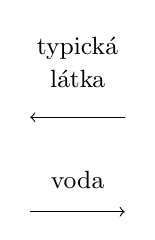
\begin{tikzpicture}
  \node[align=center] at (0,1.2) {\small typická\\ \small látka};
  \draw[<-] (-0.6,0.5) -- (0.6,0.5);
  \node at (0,-0.3) {\small voda};
  \draw[->] (-0.6,-0.7) -- (0.6,-0.7);
\end{tikzpicture}
\quad
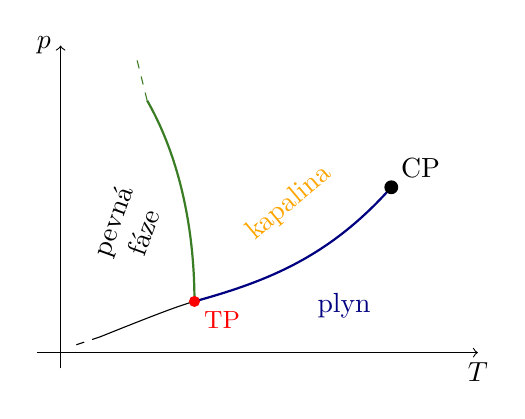
\begin{tikzpicture}[x=1cm,y=1cm]
  \draw[->] (-0.3,0) -- (5.3,0) node[below] {$T$};
  \draw[->] (0,-0.2) -- (0,3.9) node[left] {$p$};
  \draw[dashed] (0.2,0.1) -- (0.5,0.2);
  \draw (0.5,0.2) .. controls (1,0.4) and (1.5,0.6) .. (1.7,0.65);
  \draw[OliveGreen,thick] (1.7,0.65) .. controls (1.7,1.6) and (1.5,2.5) .. (1.1,3.2);
  \draw[OliveGreen,dashed] (1.1,3.2) -- (0.95,3.8);
  \draw[NavyBlue,thick] (1.7,0.65) .. controls (2.6,0.9) and (3.4,1.2) .. (4.2,2.1);
  \fill (4.2,2.1) circle (2.5pt) node[above right] {CP};
  \fill[Red] (1.7,0.65) circle (2pt) node[below right] {\small TP};
  \node[rotate=70,align=center] at (0.85,1.6) {pevná\\ fáze};
  \node[Orange,rotate=40] at (2.9,1.9) {kapalina};
  \node[NavyBlue] at (3.6,0.6) {plyn};
\end{tikzpicture}
\end{center}

%----------------------------------------------------------------------
\strana{L7-12}
\underline{Pozn:}
\begin{itemize}[nosep]
  \item mezi kapalnou a plynnou fází lze přejít bez fázového přechodu (po trajektorii, která obchází kritický bod CP) \\
        $\Rightarrow$ v jistém smyslu se jedná o jedinou \underline{tekutou fázi}
  \item v blízkosti CP řada veličin diverguje ($\kappa_T,\dots$) \\
        -- viz kritické jevy a kritické exponenty (Callen kap.\ 10, Saggion kap.\ 7.6, 8.5)
\end{itemize}

\subsection{Gibbsovo pravidlo fází}
\begin{itemize}
  \item fázová rovnováha v multi-komponentních systémech
  \item mějme $k$ chemických komponent a $\pi$ fází ve vzájemné rovnováze
  \begin{align*}
    \Rightarrow\ G &= \sum_{\vartheta=1}^{\pi}G^\vartheta(T,p,N_1^\vartheta,\dots,N_k^\vartheta)
    \overset{\color{NavyBlue}\text{extenzivita}\Rightarrow\text{Euler}}{=} \sum_{\vartheta=1}^{\pi}\sum_{j=1}^{k}\mu_j^\vartheta N_j^\vartheta \\
    &= G(T,p,N_1^1,\dots,N_1^\pi,N_2^1,\dots,N_k^\pi)
  \end{align*}
  \[ \Rightarrow\ \sum_\vartheta \dd N_j^\vartheta = 0 \qquad j = 1,\dots,k \]
  \dots\ vazby na počet molů chem.\ komponent (předp., že neprobíhají chemické reakce)
  \item $\dd G = 0 = \sum_\vartheta\sum_j\mu_j^\vartheta\,\dd N_j^\vartheta$ \\
  $\to$ $\dd N_j^\vartheta$ nejsou nezávislé $\Rightarrow$ přidám vazby prostřednictvím Lag.\ multiplikátorů $\lambda_j$:
  \[
    \dd G + \sum_j\lambda_j\sum_\vartheta\dd N_j^\vartheta = \sum_\vartheta\sum_j\big(\mu_j^\vartheta + \lambda_j\big)\dd N_j^\vartheta = 0
  \]
  \[
    \Rightarrow\ \boxed{\mu_j^\vartheta = -\lambda_j \quad j = 1,\dots,k;\ \vartheta = 1,\dots,\pi}
  \]
  \item $\lambda_j = -\mu_j^1$ $\Rightarrow$ dostáváme \underline{$k(\pi - 1)$ rovnic} popisujících vzájemnou rovnováhu $\pi$ fází v $k$-komponentním systému
  \item \underline{počet TD stupňů volnosti}: \ $G^\vartheta = G^\vartheta(T,p,N_1^\vartheta,\dots,N_k^\vartheta) = N^\vartheta g^\vartheta(T,p,c_1^\vartheta,\dots,c_k^\vartheta)$ \\
        s podmínkami $\sum_j c_j^\vartheta = 1$, $\vartheta = 1,\dots,\pi$ $\Rightarrow$ $\pi(k-1)$ koncentrací je nezávislých
  \item neboli rovnovážný stav každé fáze je určen $(k-1)$ koncentracemi chemických komponent \& $(T,p)$; $N^\vartheta$ -- počet částic v dané fázi je \uv{velikost dané domény}, nemá vliv na TD rovnováhu s okolím
\end{itemize}
\begin{veta}[Gibbsovo pravidlo fází]
\[
  \Rightarrow\ f = \underbrace{2}_{T,p} + \pi(k-1) - k(\pi - 1) \ \Rightarrow\ \vzorec{f = 2 + k - \pi}
\]
\# TD stupňů volnosti $\Leftrightarrow$ dimenze nadplochy koexistence
\end{veta}

%----------------------------------------------------------------------
\strana{L7-13}
\begin{priklad}[Př]
\begin{tabular}{@{}l@{\quad}l@{\quad}l}
$\bullet$ $k = 1$, $\pi = 2$ & $\Rightarrow$ $f = 1$ & -- křivka koexistence \\
$\bullet$ $k = 1$, $\pi = 3$ & $\Rightarrow$ $f = 0$ & -- trojný bod \\
$\bullet$ $k = 1$, $\pi = 1$ & $\Rightarrow$ $f = 2$ & -- 1-komp.\ systém v plynné fázi \\
$\bullet$ $k = 2$, $\pi = 1$ & $\Rightarrow$ $f = 3$ & -- $T$, $p$, koncentrace 1 složky
\end{tabular}
\end{priklad}

\subsection{Fázová rovnováha v dvou-složkovém systému}

\begin{minipage}{0.48\textwidth}
\begin{tikzpicture}[x=5cm,y=1cm]
  % čočka: horní T = T0 - (T0-T1)c^2, dolní T = T0 - (T0-T1)c(2-c)
  \fill[pattern=north east lines,pattern color=gray] plot[domain=0:1,samples=50] (\x,{3-2.6*\x*\x})
      -- plot[domain=1:0,samples=50] (\x,{3-2.6*\x*(2-\x)}) -- cycle;
  \draw[thick,domain=0:1,samples=50] plot (\x,{3-2.6*\x*\x});
  \draw[thick,domain=0:1,samples=50] plot (\x,{3-2.6*\x*(2-\x)});
  \draw[->] (-0.03,0) -- (1.12,0) node[right] {$c_1$};
  \draw[->] (0,-0.1) -- (0,3.6) node[left] {$T$};
  \draw[dotted] (1,0) -- (1,3.5);
  \node[below] at (0,0) {$0$}; \node[below] at (1,0) {$1$};
  \node[left] at (0,3) {$T_0$}; \node[below right] at (1,0.4) {$T_1$};
  \node at (0.25,3.4) {$p = \text{konst.}$};
  \node at (0.6,2.6) {plyn};
  \node at (0.2,0.7) {kapalina};
  % vazná přímka
  \fill ({1-sqrt(1-0.6/2.6)},1.8) circle (1.5pt) node[below left] {$l$};
  \fill ({sqrt(1.2/2.6)},1.8) circle (1.5pt) node[above right] {$g$};
  \draw[dashed] ({1-sqrt(1-0.6/2.6)},1.8) -- ({sqrt(1.2/2.6)},1.8);
  \fill[green!70!black] (0.42,1.8) circle (1.2pt);
  \node[green!70!black] at (0.42,1.5) {\small Z};
  \node[align=center,font=\tiny] at (-0.17,1.9) {teplota\\ koexistence\\ pro čistou\\ \uv{2}};
  \node[align=center,font=\tiny] at (1.0,1.0) {teplota\\ koexistence\\ pro čistou \uv{1}};
\end{tikzpicture}
\end{minipage}
\begin{minipage}{0.5\textwidth}
\begin{itemize}
  \item[--] $k = 2$, $\pi = 2$ $\Rightarrow$ $f = 2$ \dots\ plocha koexistence $\mu_1(T,p,c_1^1) = \mu_2(T,p,c_1^2)$ \\
        $c_1^\vartheta$ \dots\ koncentrace první složky ve fázi $\vartheta$
  \item[--] pro $p$ pevné, plyn je stabilní pro vysoké $T$ a kapalina pro nižší $T$
\end{itemize}
\end{minipage}

\begin{itemize}
  \item[--] šedě vyšrafovaná plocha odpovídá ploché části stabilní izotermy -- stav Z odpovídá \uv{směsi} stavů \underline{$l$} a \underline{$g$} \\
        = koexistence fází, přičemž rovnovážná koncentrace $c_1$ je \pozor{v každé fázi jiná!} (tak jako předtím mol.\ objem, \dots)
\end{itemize}

\underline{Cv:}
\begin{enumerate}[label=\arabic*)]
  \item vysvětlete na základě obrázku, proč během vypařování klesá koncentrace složky \uv{1} v kapalině
  \item Callen 9.7-1, 2 (str.\ 252) \\
  Nechť horní křivka v obrázku je popsána funkcí
  \[ T = T_0 - (T_0 - T_1)\,c_1^2 \]
  a dolní funkcí
  \[ T = T_0 - (T_0 - T_1)\,c_1(2 - c_1) \]
  Kapalina se nachází hluboko pod teplotou varu a koncentrace je na počátku $c_1 = c_2 = 1/2$.
  \begin{enumerate}[label=\alph*)]
    \item Směs uvedeme za konst.\ tlaku k varu. Jaká bude koncentrace $c_1$ v páře ve chvíli, kdy směs právě začne vařit?
    \item Je-li $\big(-\frac{\dd N}{N}\big) > 0$ úbytek látky v kapalném skupenství, ukažte, že
    \[ \dd c_1 = -\Big[\big(2c_1 - c_1^2\big)^{1/2} - c_1\Big]\Big(-\frac{\dd N}{N}\Big) \]
    je změna koncentrace \uv{1} v kap.
\end{enumerate}
\end{enumerate}

%----------------------------------------------------------------------
\strana{L7-14}
\begin{center}
\begin{tikzpicture}[x=9cm,y=0.85cm,font=\small]
  % oblasti
  \fill[pattern=north east lines] (0,5.6) .. controls (0.12,5.2) and (0.35,4.6) .. (0.47,4.0) -- (0.23,4.0) .. controls (0.15,4.6) and (0.05,5.2) .. (0,5.6);
  \fill[pattern=north east lines] (0.47,4.0) .. controls (0.6,5.0) and (0.8,6.4) .. (1,6.9) .. controls (0.9,6.4) and (0.8,5.0) .. (0.74,4.0) -- cycle;
  \fill[pattern=north west lines] (0.23,4.0) -- (0.74,4.0) -- (0.9,2.3) -- (0.96,1.1) -- (0.08,0.6) -- (0.14,2.3) -- cycle;
  % hranice
  \draw[thick] (0,5.6) .. controls (0.12,5.2) and (0.35,4.6) .. (0.47,4.0);
  \draw[thick] (0,5.6) .. controls (0.05,5.2) and (0.15,4.6) .. (0.23,4.0);
  \draw[thick] (0.47,4.0) .. controls (0.6,5.0) and (0.8,6.4) .. (1,6.9);
  \draw[thick] (0.74,4.0) .. controls (0.8,5.0) and (0.9,6.4) .. (1,6.9);
  \draw[thick] (0.23,4.0) -- (0.74,4.0);
  \draw[thick] (0.23,4.0) .. controls (0.18,3.3) and (0.12,1.8) .. (0.08,0.6);
  \draw[thick] (0.74,4.0) -- (0.9,2.3) -- (0.96,1.1);
  \draw[dashed] (0.64,5.3) -- (0.81,5.3);
  \draw[dashed] (0.14,2.3) -- (0.9,2.3);
  % osy
  \draw[thick] (0,0) -- (1,0); \draw[thick] (0,0) -- (0,6.9); \draw[thick] (1,0) -- (1,7);
  \node[below] at (0,0) {\bfseries 0}; \node[below] at (1,0) {\bfseries 1};
  \node[below] at (0.5,-0.1) {$x_1 \longrightarrow$};
  \node[left] at (-0.03,3.5) {$\uparrow T$};
  % body
  \foreach \x/\y/\l/\p in {0/5.6/B/above right, 1/6.9/A/above left, 0.47/4.0/D/below, 0.23/4.0/E/below, 0.74/4.0/C/below,
      0.64/5.3/H/above left, 0.73/5.3/G/above, 0.81/5.3/F/right, 0.9/2.3/J/right, 0.14/2.3/L/below right, 0.62/2.3/K/below}
    {\fill (\x,\y) circle (1.5pt) node[\p] {\bfseries\itshape \l};}
  \fill (0.4,5.0) circle (1.5pt) node[right] {\itshape N};
  \fill (0.05,2.1) circle (1.5pt) node[below] {\itshape Q};
  % popisky
  \node at (0.42,6.1) {Liquid};
  \node[fill=white,inner sep=1pt,align=center] at (0.24,4.6) {Liquid\\ $+\beta$};
  \node[fill=white,inner sep=1pt,align=center] at (0.66,4.6) {Liquid\\ $+\alpha$};
  \node[align=center] at (0.09,3.6) {$\beta$-phase\\ (solid)};
  \node[align=center] at (0.88,4.4) {$\alpha$-phase\\ (solid)};
  \node[fill=white,inner sep=1pt] at (0.46,3.2) {$\alpha + \beta$};
  \node at (0.07,6.6) {$p = \text{konst.}$};
  \node[NavyBlue,align=center] at (0.62,7.3) {liquid (H)\\ + solid (F)};
  \draw[NavyBlue,->] (0.66,6.75) -- (0.72,5.45);
  \node[NavyBlue,align=center] at (0.76,1.0) {solid (L)\\ + solid (J)};
  \draw[NavyBlue,->] (0.7,1.45) -- (0.63,2.15);
\end{tikzpicture}
\hspace{0.3cm}
\begin{minipage}[b]{0.3\textwidth}
Typický fázový diagram \underline{kapalina -- pevná fáze} v dvousložkovém systému

{\color{NavyBlue}
viz Callen 250 $\to$ \\
viz Michael Cross \\
{\small\url{http://www.pmaweb.caltech.edu/~mcc/Ph127/index.html}} \\
(2nd term, Lectures 3, 4)}
\vspace{2cm}
\end{minipage}
\end{center}

